\begin{savequote}[45mm]
\ascii{Any fool can write code that a computer can understand. Good programmers write code that humans can understand.}
\qauthor{\ascii{- Martin Flower}}
\end{savequote}

\chapter{介绍} 
\label{ch:introduction}

\begin{content}

\ascii{TensorFlow}是一个支持大规模和异构环境的机器学习系统。它使用\emph{数据流图}\ascii{(Dataflow Graph)}表示计算过程和共享状态,使用节点表示抽象计算,使用边表示数据流。\upcite{tf-white-paper}

数据流图的节点被映射在集群中的多个机器,在一个机器内被映射在多个计算设备\ascii{(Device)}上,包括\ascii{CPU, GPU, TPU}。\ascii{TensorFlow}灵活的架构支持多种计算平台,包括台式机,服务器,移动终端等。

\tf{}最初由\ascii{Google Brain}的研究员和工程师们开发出来,用于开展机器学习和深度神经网络方面的研究,但\tf{}优异的通用性使其也可广泛用于其他领域的数值计算。

\end{content}

\section{前世今生}

\begin{content}

\tf{}是\ascii{DistBelief}的后继者,它站在巨人的肩膀上,革命性地重新设计架构设计,使得\tf{}在机器学习领域一鸣惊人,在社区中产生了重大的影响。

为了更好地理解\tf{}系统架构的优越性,得先从\ascii{DistBelief}谈起。

\end{content}

\subsection{DistBelief}

\begin{content}

\ascii{DistBelief}是一个用于训练大规模神经网络的的分布式系统,是\ascii{Google}第一代分布式机器学习框架。自\ascii{2011}年以来,在\ascii{Google}内部大量使用\ascii{DistBelief}训练大规模的神经网络。

\end{content}

\subsubsection{编程模型}

\begin{content}

\ascii{DistBelief}的编程模型是基于层\ascii{(Layer)}的\ascii{DAG(Directed Acyclic Graph)}图。层可以看做是一种组合多个运算操作符的复合运算符,它完成特定的计算任务。

例如,全连接层完成$f({W^T}x + b)$的复合计算,包括输入与权重的矩阵乘法,随后再与偏置相加,最后在线性加权值的基础上实施非线性变换。

\end{content}

\subsubsection{架构}

\begin{content}

\ascii{DistBelief}使用参数服务器\ascii{(Parameter Server)}的系统架构,训练作业包括两个分离的进程:无状态的\ascii{Worker}进程,用于模型训练的计算;有状态的\ascii{PS(Parameter Server)}进程,用于维护模型参数。

如\refig{parameter-server}所示,在分布式训练过程中,各个模型备份\ascii{(Model Relica)}异步地从\ascii{PS}上拉取\ascii{(Fetch)}训练参数$w$,当完成一步迭代运算后,推送\ascii{(Push)}参数的梯度$ \nabla w $到\ascii{PS}上去,并完成参数更新。

\begin{figure}[!htbp]
\centering
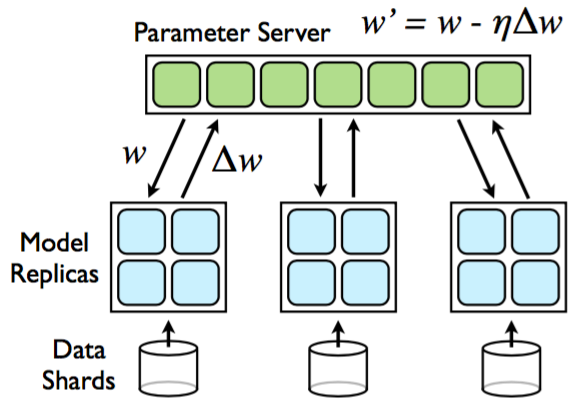
\includegraphics[width=0.6\textwidth]{figures/parameter-server.png}
\caption{DistBelief: Parameter Server架构}
 \label{fig:parameter-server}
\end{figure}

\end{content}

\subsubsection{缺陷}

\begin{content}


但是,对于高级用户,\ascii{DistBelief}的编程模型,及其\ascii{Parameter Server}的系统架构,缺乏如下几个方面的扩展性。

\begin{enum}
  \eitem{优化算法:添加新的优化算法,必须修改\ascii{Parameter Server}的实现;\code{get(), put()}的抽象方法,对某些优化算法并不高效;}
  \eitem{训练算法:支持非前馈的神经网络具有很大的挑战性,例如包含循环的\ascii{RNN},交替训练的对抗网络,及其损失函数由分离的代理完成增强学习模型;} 
  \eitem{加速设备:\ascii{DistBelief}设计之初仅支持多核\ascii{CPU},并不支持\ascii{GPU};遗留的系统架构对支持新的计算设备缺乏弹性空间。}
\end{enum}

\end{content}

\subsection{TensorFlow}

\begin{content}

正因为\ascii{DistBelief}遗留的架构和设计,不再满足潜在的深度学习与日俱增的需求,\ascii{Google}毅然决定在\ascii{DistBelief}基础上做全新的架构设计,从而诞生了\ascii{TensorFlow}。

\end{content}

\subsubsection{编程模型}

\begin{content}

\ascii{TensorFlow}使用数据流图\ascii{(Dataflow Graph)}表示计算过程和共享状态,使用节点表示抽象计算,使用边表示数据流。如\refig{tf-dataflow}所示,展示了\ascii{mnist}手写识别应用的数据流图。

在该模型中,前向子图使用了\ascii{2}层全连接网络,分别为\ascii{ReLU}层和\ascii{Softmax}层;随后,由\ascii{Gradients}构建了与前向子图对应的反向子图,用于训练参数的梯度计算;最后,使用`SGD`的优化算法,构造参数更新子图,完成参数的更新。

\begin{figure}[!htbp]
\centering
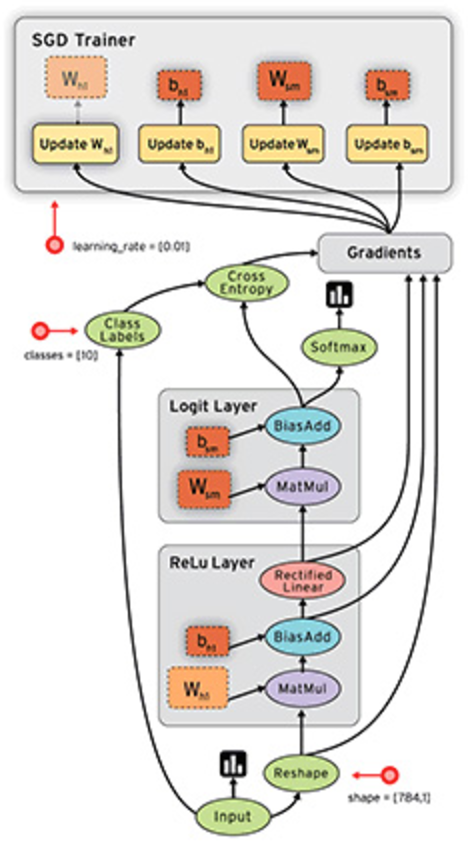
\includegraphics[width=0.4\textwidth]{figures/tf-dataflow.png}
\caption{TensorFlow数据流图}
 \label{fig:tf-dataflow}
\end{figure}

\end{content}

\subsubsection{设计原则}

\begin{content}

\begin{enum}
  \eitem{延迟计算:图的构造与执行分离,并推迟计算图的执行过程;}
  \eitem{原子\ascii{OP}:\ascii{OP}是最小的抽象计算单元,支持构造复杂的网络模型;} 
  \eitem{抽象设备:支持\ascii{CPU, GPU, TPU}多种异构计算设备类型;}
  \eitem{抽象任务:基于\ascii{Task}的\ascii{PS}任务,对新的优化算法和网络模型具有良好的可扩展性。}  
\end{enum}

\end{content}

\subsubsection{优势}

\begin{content}

相对于其他机器学习框架,\ascii{TensorFlow}具有如下方面的优势。

\begin{enum}
  \eitem{跨平台:支持多\ascii{CPU/GPU/TPU}运算;支持台式机/服务器/移动设备;支持\ascii{Windows,Linux,MacOS};}
  \eitem{分布式:支持本地和分布式的模型训练和推理;}
  \eitem{多语言:支持\ascii{Python, C++, Java, Go}等多种程序设计语言的\ascii{API};}  
  \eitem{通用性:支持各种复杂的网络模型的设计和实现;}
  \eitem{可扩展:支持\ascii{OP}扩展,\ascii{Kernel}扩展,\ascii{Device}扩展;}
  \eitem{可视化:使用\ascii{TensorBoard}可视化整个训练过程,包括计算图。}
\end{enum}

\end{content}

\section{社区发展}

\begin{content}

\tf{}是目前最为流行的机器学习框架。自开源以来,\tf{}社区相当活跃。来自众多的非\ascii{Google}员工拥有数万次代码提交,并且每周拥有近百个\ascii{Issue}被提交;在\ascii{Stack Overflow}上也拥有上万个关于\tf{}的问题被回答;在各类技术大会上,\tf{}也是一颗闪亮的明星,得到众多开发者的青睐。

\end{content}

\subsection{开源}

\begin{content}

\ascii{2015.11},\ascii{Google Research}发布文章:\href{https://research.googleblog.com/2015/11/tensorflow-googles-latest-machine\_9.html}{TensorFlow: Google's latest machine learning system, open sourced for everyone},正式宣布新一代机器学习系统\ascii{TensorFlow}开源。

随后,\ascii{TensorFlow}在\ascii{Github}上代码仓库短时间内获得了大量的\ascii{Star}和\ascii{Fork}。如\refig{tf-commits}所示,\ascii{TensorFlow}的社区活跃度已远远超过其他竞争对手,逐渐成为目前最为炙手可热的机器学习和深度学习框架,已然成为事实上的工业标准。

\begin{figure}[!htbp]
\centering
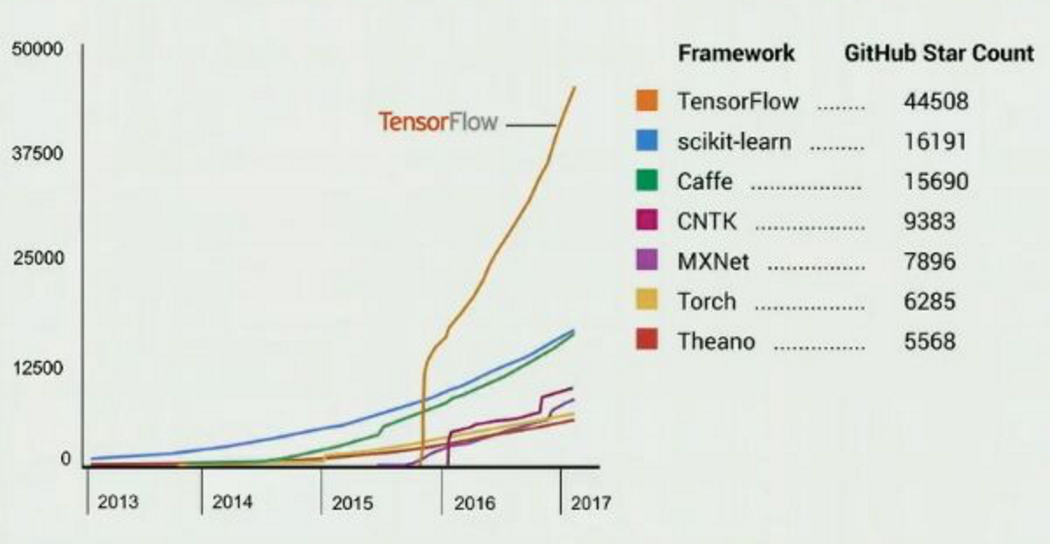
\includegraphics[width=1.0\textwidth]{figures/tf-commits.png}
\caption{TensorFlow社区活跃度}
 \label{fig:tf-commits}
\end{figure}

毫无疑问,\ascii{TensorFlow}的开源对学术界和工业界产生了巨大的影响,其极大地降低了深度学习在各个行业中应用的难度。众多的学者,工程师,企业,组织纷纷地投入到了\ascii{TensorFlow}社区,并一起完善和改进\ascii{TensorFlow},推动其不断地向前演进和发展。

\end{content}

\subsection{里程碑}

\begin{content}

\tf{}自\ascii{2015.11}开源依赖,平均一个多月发布一个版本。如\refig{tf-versions}所示,展示了\tf{}几个重要特性的发布时间。

\begin{figure}[!htbp]
\centering
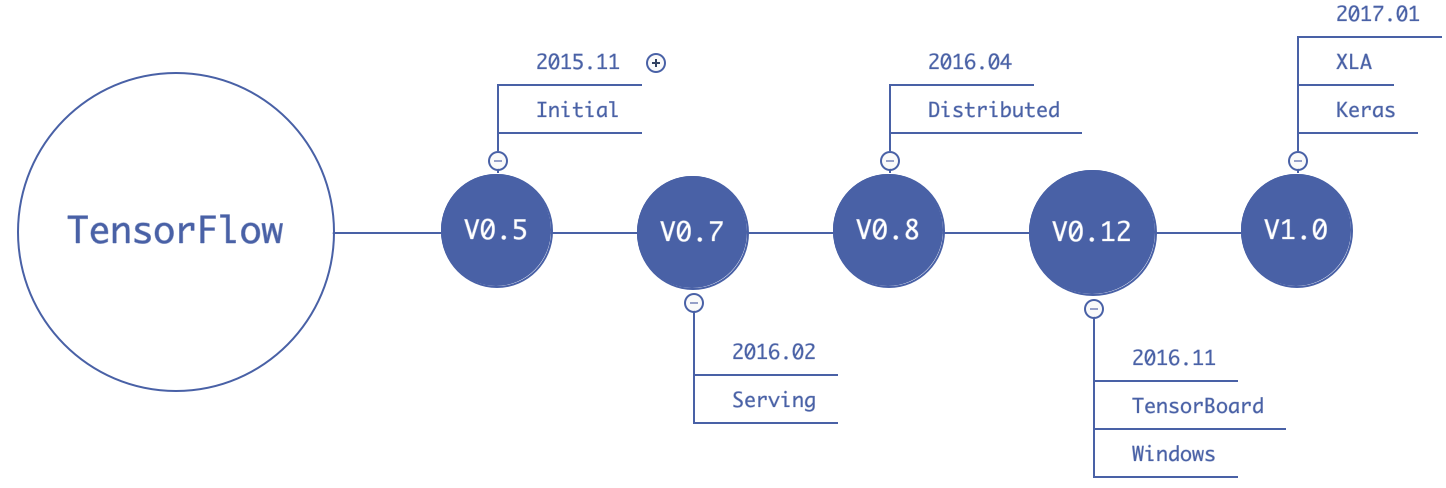
\includegraphics[width=1.0\textwidth]{figures/tf-versions.png}
\caption{TensorFlow重要里程碑}
 \label{fig:tf-versions}
\end{figure}

\end{content}

\subsection{工业应用}

\begin{content}

\ascii{TensorFlow}自开源发展一年多以来,在生产环境中被大量应用使用。在医疗方面,使用\ascii{TensorFlow}构建机器学习模型,帮助医生预测皮肤癌;在音乐、绘画领域,使用\ascii{TensorFlow}构建深度学习模型,帮助人类更好地理解艺术;在移动端,多款移动设备搭载\ascii{TensorFlow}训练的机器学习模型,用于翻译等工作。

如\refig{tf-google-apps}所示,\ascii{TensorFlow}在\ascii{Google}内部项目应用的增长也十分迅速,多个产品都有相关应用,包括:\ascii{Search, Gmail, Translate,  Maps}等等。

\begin{figure}[!htbp]
\centering
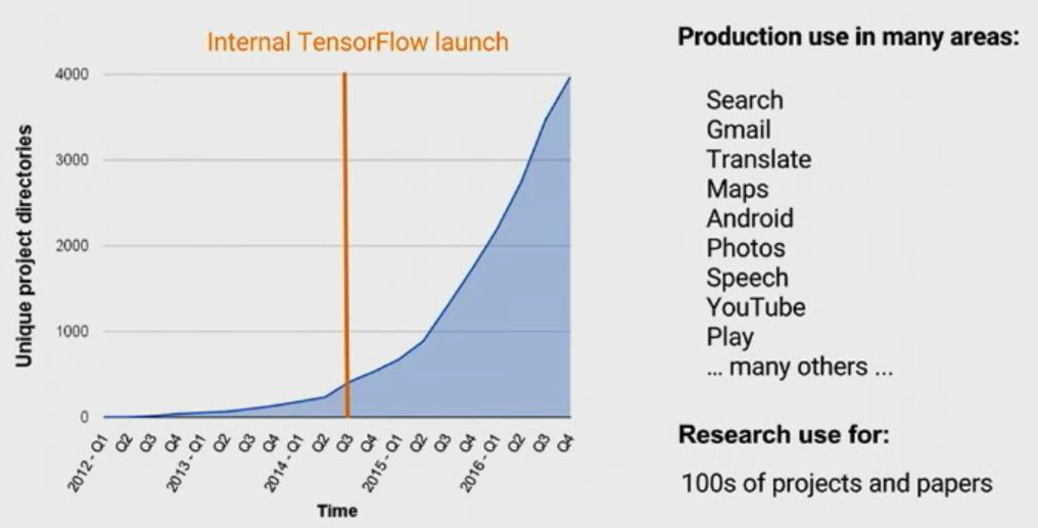
\includegraphics[width=1.0\textwidth]{figures/tf-google-apps.png}
\caption{TensorFlow在Google内部使用情况}
 \label{fig:tf-google-apps}
\end{figure}


\end{content}